\documentclass{standalone}
\usepackage{PhysicalChemistryNote}
\begin{document}
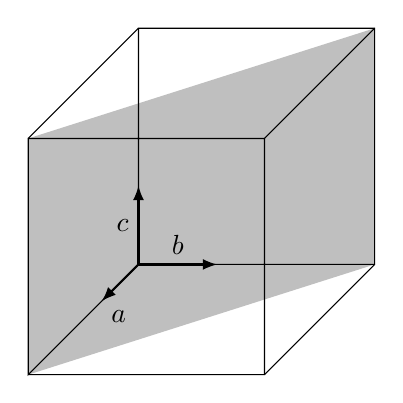
\begin{tikzpicture}
    \fill[rectangle,gray,opacity=0.5] (0,0)--(4.4,1.4)--(4.4,4.4)--(0,3);
    \draw[-] (0,0)--(3,0)--(3,3)--(0,3)--(0,0)--(1.4,1.4)--(1.4,4.4)--(4.4,4.4)--(4.4,1.4)--(1.4,1.4);
    \draw[-] (3,0)--(4.4,1.4);
    \draw[-] (0,3)--(1.4,4.4);
    \draw[-] (3,3)--(4.4,4.4);
    \draw[-latex,thick] (1.4,1.4)--(0.933,0.933);\node[below right] at (0.933,0.933) {$\mbf a$};
    \draw[-latex,thick] (1.4,1.4)--(2.4,1.4);\node[above] at (1.9,1.4) {$\mbf b$};
    \draw[-latex,thick] (1.4,1.4)--(1.4,2.4);\node[left] at (1.4,1.9) {$\mbf c$};
\end{tikzpicture}
\end{document}